%%%% ijcai25.tex

\typeout{IJCAI--25 Instructions for Authors}

% These are the instructions for authors for IJCAI-25.

\documentclass{article}
\pdfpagewidth=8.5in
\pdfpageheight=11in

% The file ijcai25.sty is a copy from ijcai22.sty
% The file ijcai22.sty is NOT the same as previous years'
\usepackage{ijcai25}

% Use the postscript times font!
\usepackage{times}
\usepackage{soul}
\usepackage{url}
\usepackage[hidelinks]{hyperref}
\usepackage[utf8]{inputenc}
\usepackage[small]{caption}
\usepackage{graphicx}
\usepackage{amsmath}
\usepackage{amsthm}
\usepackage{booktabs}
\usepackage{algorithm}
\usepackage{algorithmic}
\usepackage[switch]{lineno}

\usepackage{my}
% cys
\usepackage[table]{xcolor}
\usepackage{colortbl}
\usepackage{makecell} % 用于多行单元格

\usepackage{makecell}
\usepackage{multirow}
\usepackage{amssymb}
\usepackage{mathrsfs}



% Comment out this line in the camera-ready submission
\linenumbers

\urlstyle{same}

% the following package is optional:
%\usepackage{latexsym}

% See https://www.overleaf.com/learn/latex/theorems_and_proofs
% for a nice explanation of how to define new theorems, but keep
% in mind that the amsthm package is already included in this
% template and that you must *not* alter the styling.


% Following comment is from ijcai97-submit.tex:
% The preparation of these files was supported by Schlumberger Palo Alto
% Research, AT\&T Bell Laboratories, and Morgan Kaufmann Publishers.
% Shirley Jowell, of Morgan Kaufmann Publishers, and Peter F.
% Patel-Schneider, of AT\&T Bell Laboratories collaborated on their
% preparation.

% These instructions can be modified and used in other conferences as long
% as credit to the authors and supporting agencies is retained, this notice
% is not changed, and further modification or reuse is not restricted.
% Neither Shirley Jowell nor Peter F. Patel-Schneider can be listed as
% contacts for providing assistance without their prior permission.

% To use for other conferences, change references to files and the
% conference appropriate and use other authors, contacts, publishers, and
% organizations.
% Also change the deadline and address for returning papers and the length and
% page charge instructions.
% Put where the files are available in the appropriate places.


% PDF Info Is REQUIRED.

% Please leave this \pdfinfo block untouched both for the submission and
% Camera Ready Copy. Do not include Title and Author information in the pdfinfo section
\pdfinfo{
/TemplateVersion (IJCAI.2025.0)
}

\title{CABTO: Context-Aware Behavior Tree Grounding for Robot Manipulation}


% Single author syntax
\author{
    Author Name
    \affiliations
    Affiliation
    \emails
    email@example.com
}


\begin{document}

\maketitle

\begin{abstract}
% 行为树是机器人领域的一个重要控制架构,具有模块化、层次化、反应性等优点。行为树被证明是可自动规划的,这有利于机器人的自主完成任务。然而,行为树的动作节点通常需要人类专家精心设计,从而保证能够可靠执行,并让环境产生正确的转移。本文关注于无须大量专家设计的行为树的底层控制,提出了一种context-aware behavior tree grounding(CABTO)方法,根据节点邻居、历史动作、未来动作、当前感知等上下文信息来让Vision-language models (VLMs) 输入行为树节点的执行代码。CABTO方法不仅能够实现节点的自动控制,还能基于反应式反馈来实现行为树验证和纠错,从而保证行为树执行的鲁棒性。We present system implementations on both single-arm  and dual-arm platforms, 结果表明CABTO能够很好地执行行为树节点。

Behavior trees (BTs) are becoming a popular control architecture for robots, featuring modularity, reactivity and robustness. BT planning, an emerging approach, provides theoretical guarantee to generate reliable BTs for achieving tasks automatically. However, current BT planning methods often rely on a well-designed BT system, which require expensive expert knowledge to construct both high-level action models and low-level behavior control. This paper proposes the first framework for automatically designing and grounding a BT system based on the task and execution contexts, named Context-Aware Behavior Tree grOunding (CABTO). CABTO includes two phases: forward and feedback. In the forward phase, we utilize Large Language Models (LLMs) for BT system designing, formal algorithms for BT planning and Vision-Language Models (VLMs) for BT execution. If any failure occurs, the pipeline immediately transitions to the feedback phase, where each reported error will be corrected based on the contexts. CABTO integrates pre-trained large models with formal verification, thus achieving both generalization and reliability. We construct experiments on 4 household scenarios and 10 manipulation tasks with the Fetch robot. The results shows the CABTO is a general and reliable for automatic BT system grounding and task execution.


% to generate chunked target poses for motion planning based on contextual information. The contexts includes node neighbors, history actions, future actions, and current perception, etc. CABTO not only enables automatic node control but also achieves BT verification and error correction based on reactive feedback, ensuring robust execution of BTs. We present system implementations on both single-arm and dual-arm platforms, with results demonstrating that CABTO can effectively execute BT nodes without task-specific data or environment models.

\end{abstract}


% The symbolic system is a subset of language, but more realiable and disambiguas with clear definitions and action models.

% We introduce a new family of embodied foundation models named Vision-Symbolic-Action Model (VSA). To solve the symbolic grounding problem, we present Symbolic VLA, a hierarchical Vision-Language-Action (VLA) policy for robotic manipulation tasks.

% There are lots of work to study the PDDL automated generating \cite{liu2023llm,mahdavi2024leveraging}.



\section{Introduction}

% 机器人的操作的任务即需要灵活的场景理解、可靠而鲁棒的任务规划以及灵活可行的底层执行。近年来,行为树被证明是一个可靠的机器人控制架构,以safety,robustness,模块化和反应性出名。一方面,行为树的模块化本质使得每个行为节点的设计变得更加容易和可控;另一方面,在有了formal modeling of the 行为树系统之后,就可以通过BT planning algorithms来自动生成并验证可达成目标的可靠行为树。

Robot manipulation requires accurate task understanding, reliable and robust task planning, and flexible and feasible motion control. In recent years, behavior trees (BTs) \cite{colledanchise2018behavior,ogren2022behavior} have proven to be a reliable robot control architecture, known for safety, robustness, modularity, and reactivity \cite{colledanchise2019blended,colledanchise2016how}. On one hand, the modular nature of BTs makes the design of each behavior node easier and assemble them together to make a whole policy more easier; on the other hand, with the formal modeling of the BT system, reliable BTs that achieve the desired goals can be automatically generated and verified through BT planning algorithms \cite{cai2021bt,chen2024integrating,cai2025mrbtp}.


% One of the main goals of robotics and AI is to develop intelligent robots capable of autonomously making decisions and executing behaviors in the real world. That requires not only intelligent planning algorithms, but also a safe and robust control architecture, which is particularly crucial for everyday service robots. Behavior Trees (BTs) become a popular control architecture for robots exactly due to their ability to ensure safety and robustness\cite{colledanchise2018behavior,ogren2022behavior}. Because of their modular and adaptable tree structure, BTs can effectively perform various tasks and handle uncertain environments \cite{colledanchise2019blended,colledanchise2016how}. In addition, their clear and interpretable control flows enhance the reliability and predictability of robot behavior, making BT systems easy for humans to design, deploy, and scale.


\begin{figure}[t]
    \centering
    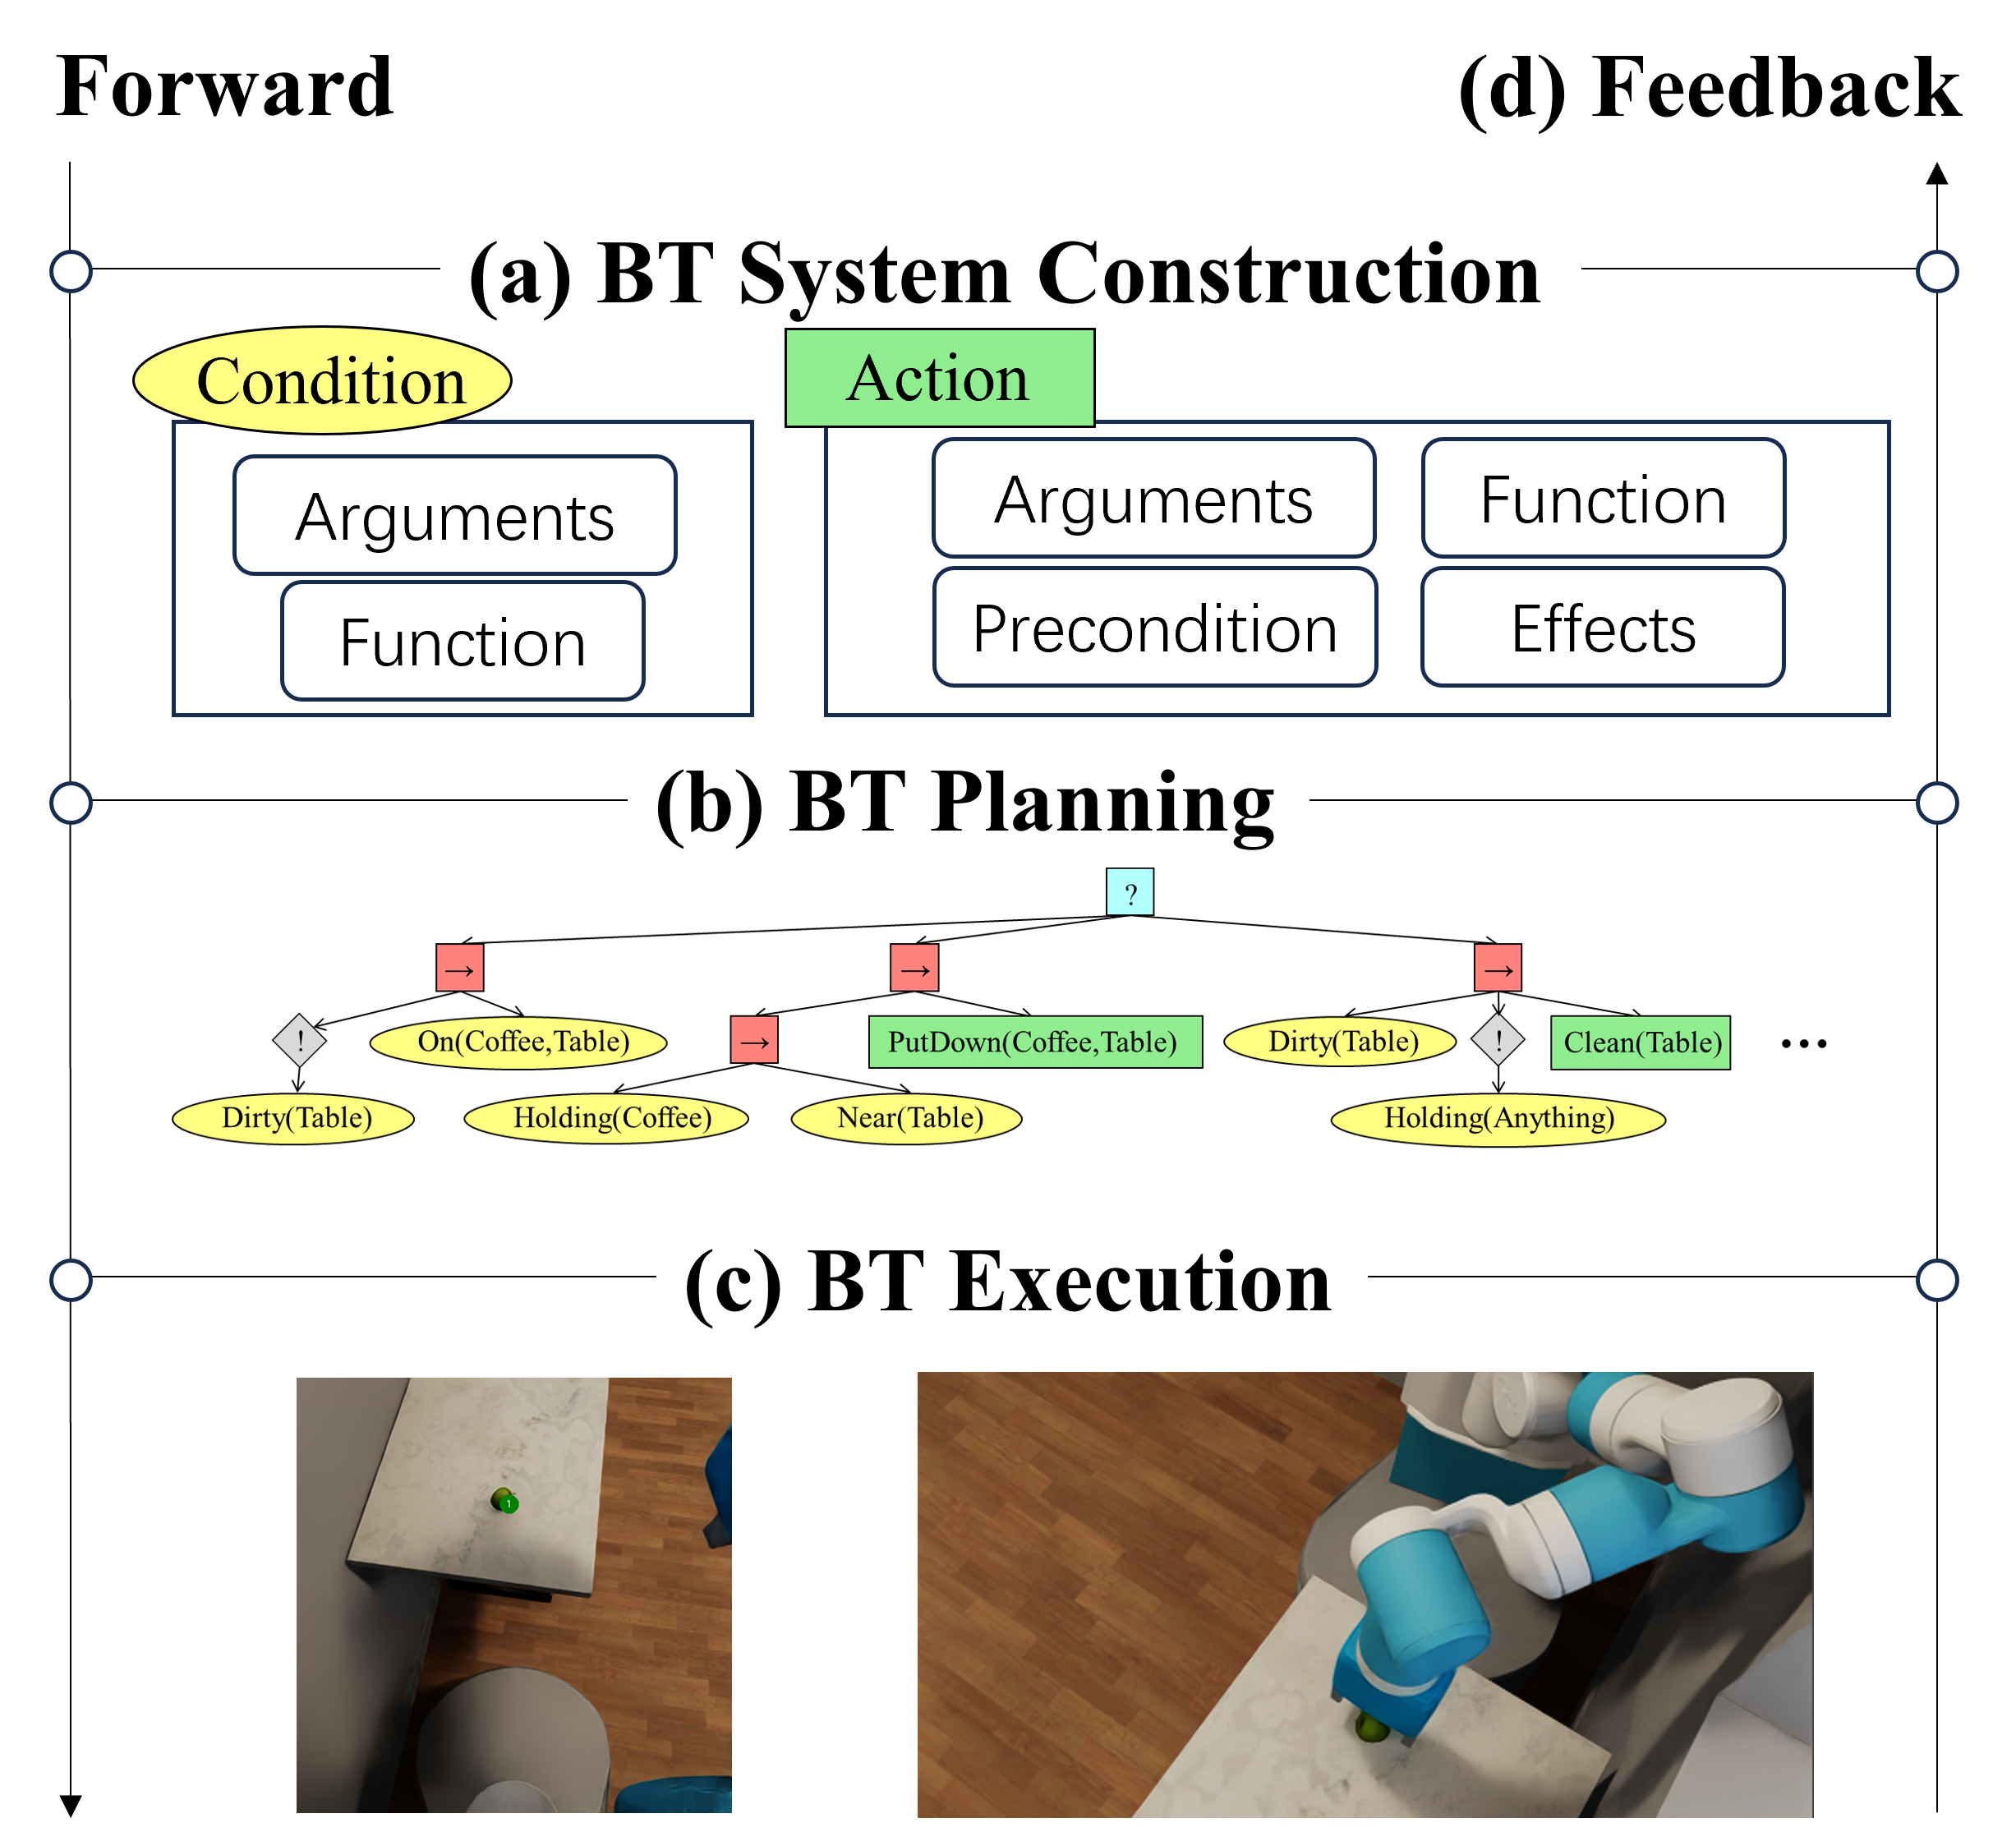
\includegraphics[width=0.5\textwidth]{figures/introduction}
    \caption{An example of CABTO procedure for the given task set. (a) BT system designing. (b) BT planning. (c) BT execution. (d) Feedback.}
    \label{fig:introduction}
\end{figure}


However, traditional BT system construction often requires substantial human expertise. For high-level BT planning, an action model based on the region of attraction (ROA) of the action node is essential. The accuracy with which experts can model the environmental transitions caused by actions determines whether BT planning algorithms can generate correct and reliable BTs. For low-level BT control, a program for each node to execute is required to ensure that the actions follow the model. Although behavior nodes are reusable across different tasks, it is inevitable that task-specific behavior trees need to be constructed to be coherent and non-redundant in order to achieve efficient planning and execution. Moreover, relying solely on traditional rule-based methods for low-level motion control makes it difficult to generalize to unseen tasks, as it is impossible to enumerate all motion control rules to cover every possible scenario in the embodied world.



This paper proposes the first framework for automatically designing and grounding a BT system based on the task and execution contexts, named Context-Aware Behavior Tree grOunding (CABTO). CABTO includes two phases: forward and feedback. In the forward phase, we utilize Large Language Models (LLMs) for BT system designing, formal algorithms for BT planning and Vision-Language Models (VLMs) for BT execution. If any failure occurs, the pipeline immediately transitions to the feedback phase, where each reported error will be corrected based on the contexts.



See Fig. \ref{fig:introduction} as an example. The task set includes 10 tasks for everyday service robots. We input the task information as the context into the LLM (Fig. \ref{fig:introduction}a). Then the LLM output we need a BT system that has condition nodes such as  \constant{IsGrasping}, \constant{IsOpen} and action nodes such as \constant{Grasp}, \constant{Open}. Then, the LLM is called again for each node to determine there node arguments and details and action models. After designing the BT system, the BT planning algorithms are applied (Fig. \ref{fig:introduction}b) for each task in the task set. When use an sound and complete algorithm, the success result indicate the BT system is coherent, thus divaricate the BT system. Then we can perform these (Fig. \ref{fig:introduction}c) to form tasks. For example for the \constant{Open}, the molmo point the handle of the cabinet in the robot's view, then the point will be converted to the world coordination.T hen the motion planning solver will be applied to finish the node execution. If failures occur, feedback will be performed (Fig. \ref{fig:introduction}d). For example, if the pose are not reachable by the motion planning, may be the node design is wrong, then the LLM will reproduce the node code for correction.

CABTO integrates pre-trained large models with formal verification, thus achieving both generalization and reliability. We construct experiments on 4 household scenarios and 10 manipulation tasks with the Fetch robot. The results shows the CABTO is a general and reliable for automatic BT system grounding and task execution.




% LLM planning \cite{song2023llmplanner} is a good way to achieve long-horizon manipulation tasks.

% Hierarchical VLA \cite{cai2024rocket1} is a good way to achieve long-horizon manipulation tasks.


% \paragraph{Symbolic reasoning} Symbolic reasoning is a good way to achieve long-horizon manipulation tasks. The symbolic system is proven help for morden AI such as visual activity understanding \cite{wu2024symbolllm}, reinforcement learning \cite{sreedharan2023optimistic}, objects and relations reasoning \cite{hsu2023ns3d}, expression recognition \cite{li2024softened,sun2022symbolic,mundhenk2021symbolic}. 

% Neural-symbolic methods \cite{sreedharan2023optimistic,mao2022pdsketch} to learning the symbolic system.


% some work use a MLP for certain concept \cite{hsu2023whats}.

% The symbolic system is a subset of language, but more realiable and disambiguas with clear definitions and action models.

% Our main contributions are as follows:
% \begin{itemize}
%     \item We propose a hierarchical reasoning framework for long-horizon robotic manipulation tasks, PDDL-VLM-Policy. 
%     \item We propose a new long-horizon task planning network with action chunking, as well as the data collection pipeline and the dataset. With feedback.
%     \item We train our model on the 10000 collected data, and evaluate it on 100 tasks, results showing that our model can achieve 90\% success rate.
% \end{itemize}


\section{Background}

\paragraph{Behavior Tree}

A BT is a directed rooted tree that consists of execution nodes and control flow nodes. Execution nodes interact with the environment, while control flow nodes handle the triggering logic of their children \cite{colledanchise2018behavior}. At each time step, the BT ticks from its root. The tick then goes through the control flow nodes to determine which action will be performed by the robot according to the environment state. The four basic BT nodes determine the return value according to the following logic:
\begin{itemize}
\item \textbf{Condition}: An execution node that checks the environment state and returns {\ttfamily success} if it satisfies the specified situation; otherwise, it returns {\ttfamily failure}.
\item \textbf{Action}: An execution node that performs a specified behavior and returns {\ttfamily success}, {\ttfamily failure}, or {\ttfamily running} depending on the execution results.
\item \textbf{Sequence}: A control flow node that ticks its children from left to right. If all its children succeed, it returns {\ttfamily success}. Otherwise, it returns {\ttfamily failure} or {\ttfamily running} if one of its children returns such a value.
\item \textbf{Fallback}: A control flow node that also ticks its children from left to right. It returns {\ttfamily failure} if all of its children fail. Otherwise, it returns {\ttfamily success} or {\ttfamily running} if one of its children returns such a value.
\end{itemize}


\paragraph{BT System}

A BT system $\Phi$ $\phi$ $\psi$ $\Psi$ $\varphi$ $\varphi$
In BT planning for a single robot \cite{cai2021bt}, we represent a BT as a three-tuple $\mathcal{T} = <f, r, \Delta t>$. $f:2^{n}\rightarrow 2^{n}$ is its effect on the environment state, $\Delta t$ is the time step, and $r:2^{n}\mapsto \{ $\constant{S}, \constant{R}, \constant{F}\} partitions states into three regions, where $\mathcal{T}$ returns success, running, failure, respectively.

Then the BT planning problem can be described as: \(<\mathcal{S},\mathcal{L},\mathcal{A},\mathcal{M}, s_0,g>\), where \( \mathcal{S} \) is the finite set of environment states, $\mathcal{L}$ is the finite set of literals that form states, \( \mathcal{A} \) is the finite set of actions, $\mathcal{M}$ is the action model, $s_0$  is the initial state, $g$ is the goal condition. 


A condition $c$ in BT is usually a subset of a state $s$. If $c\subseteq s$, it is said condition $c$ holds in that state $s$. The state transition affected by action $a\in \mathcal{A}$ can be defined as a triplet \( \mathcal{M}(a)=<pre(a),add(a),del(a)> \), comprising the precondition, add effects, and delete effects of the action. If $a$ is finished after $k$ time step, the subsequent state $s_{t'}$ will be:
\begin{equation}\label{eqn:s_f}
	s_{t'}=f_a(s_t)=s_t\cup add(a)\setminus del(a), t'=t + k
\end{equation}


\section{Problem Formulation}
We first extend the BT representation from a single robot to a multi-robot system. 

\begin{definition}[BT System]
A $n$-robot BT system is a four-tuple $\left<\Phi, f_\Phi, r_\Phi, \Delta t_\Phi\right>$, where $\Phi = \left\{ \mathcal{T}_i \right\}_{i=1}^n$ is the set of BTs, $f_\Phi: \mathcal{S} \mapsto \mathcal{S}$ is the team state transition function, $\Delta t_\Phi$ is the team time step, $r_\Phi: \mathcal{S} \mapsto \{$ \constant{S}, \constant{R}, \constant{F} $\}$ is the team region partition.
\end{definition}
Due to variability in hardware performance, we allow each robot's BT to have a different response frequency, with $\Delta t_\Phi$ representing the common minimum response interval. The state transition can be calculated as follows:
\begin{align}
    s_{t+\Delta t_\Phi} = f_\Phi(s_t) = s_t \cup \bigcup_{i=1}^n \left( add(a_i) \setminus del(a_i) \right)
\end{align}
where $a_i$ is the action of robot $i$ in time $t$. If robot $i$ does not have an action or its action is running, we let $add(a_i) = del(a_i) = \emptyset$. 

\begin{definition}[Finite Time Successful]
$\Phi$ is finite time successful (FTS) from region of attraction (ROA) $R$ to condition $c$, if $\forall s_0 \in R$  there is 
 a finite time $\tau$ such that for any $t<\tau$, $r_\Phi(s_t)=$ \constant{R}, and for any $t\geq\tau, r_\Phi(s_t)=$ \constant{S}, $c\in s_t$.
\end{definition}
With definitions above, the multi-robot BT planning problem can finally be defined.

\begin{definition}[Completeness]
A BT system is complete, iff for all tasks, produce a BT that can solve the task.
\end{definition}

\begin{definition}[Consistency]
An action node $a$ is consistent, if $r_{a}=R$ when $pre(a) \in s_t$, $s_{t+1}=s_t\cup add(a) \setminus del(a)$. A BT system with action set $\mathcal{A}$ is consistent, if $\forall a\in \mathcal{A}, a$ is consistent.
\end{definition}



\begin{definition}[Task]
A task is a tree tuple $\left<\mathcal{S}, s_0, g\right>$, where $\mathcal{S}$ is the finite state set, $s_0$ is the initial state, $g$ is the goal condition.
\end{definition}



\begin{problem}[BT Grounding]
The problem is a tuple \(\left<\mathcal{T},\mathcal{P}_c\right>\), where \( \mathcal{T} \) is the finite task set, $\mathcal{P}_c$ is the finite condition predicates. A solution to this problem is a BT system $\Phi$ which is consistent and complete in the task.

% , and for all $s$ in the team success region $S=\{s|r_\Phi(s)=$\constant{S}$\}$, $g\subseteq s$).
\end{problem}



\begin{figure*}[t]
    \centering
    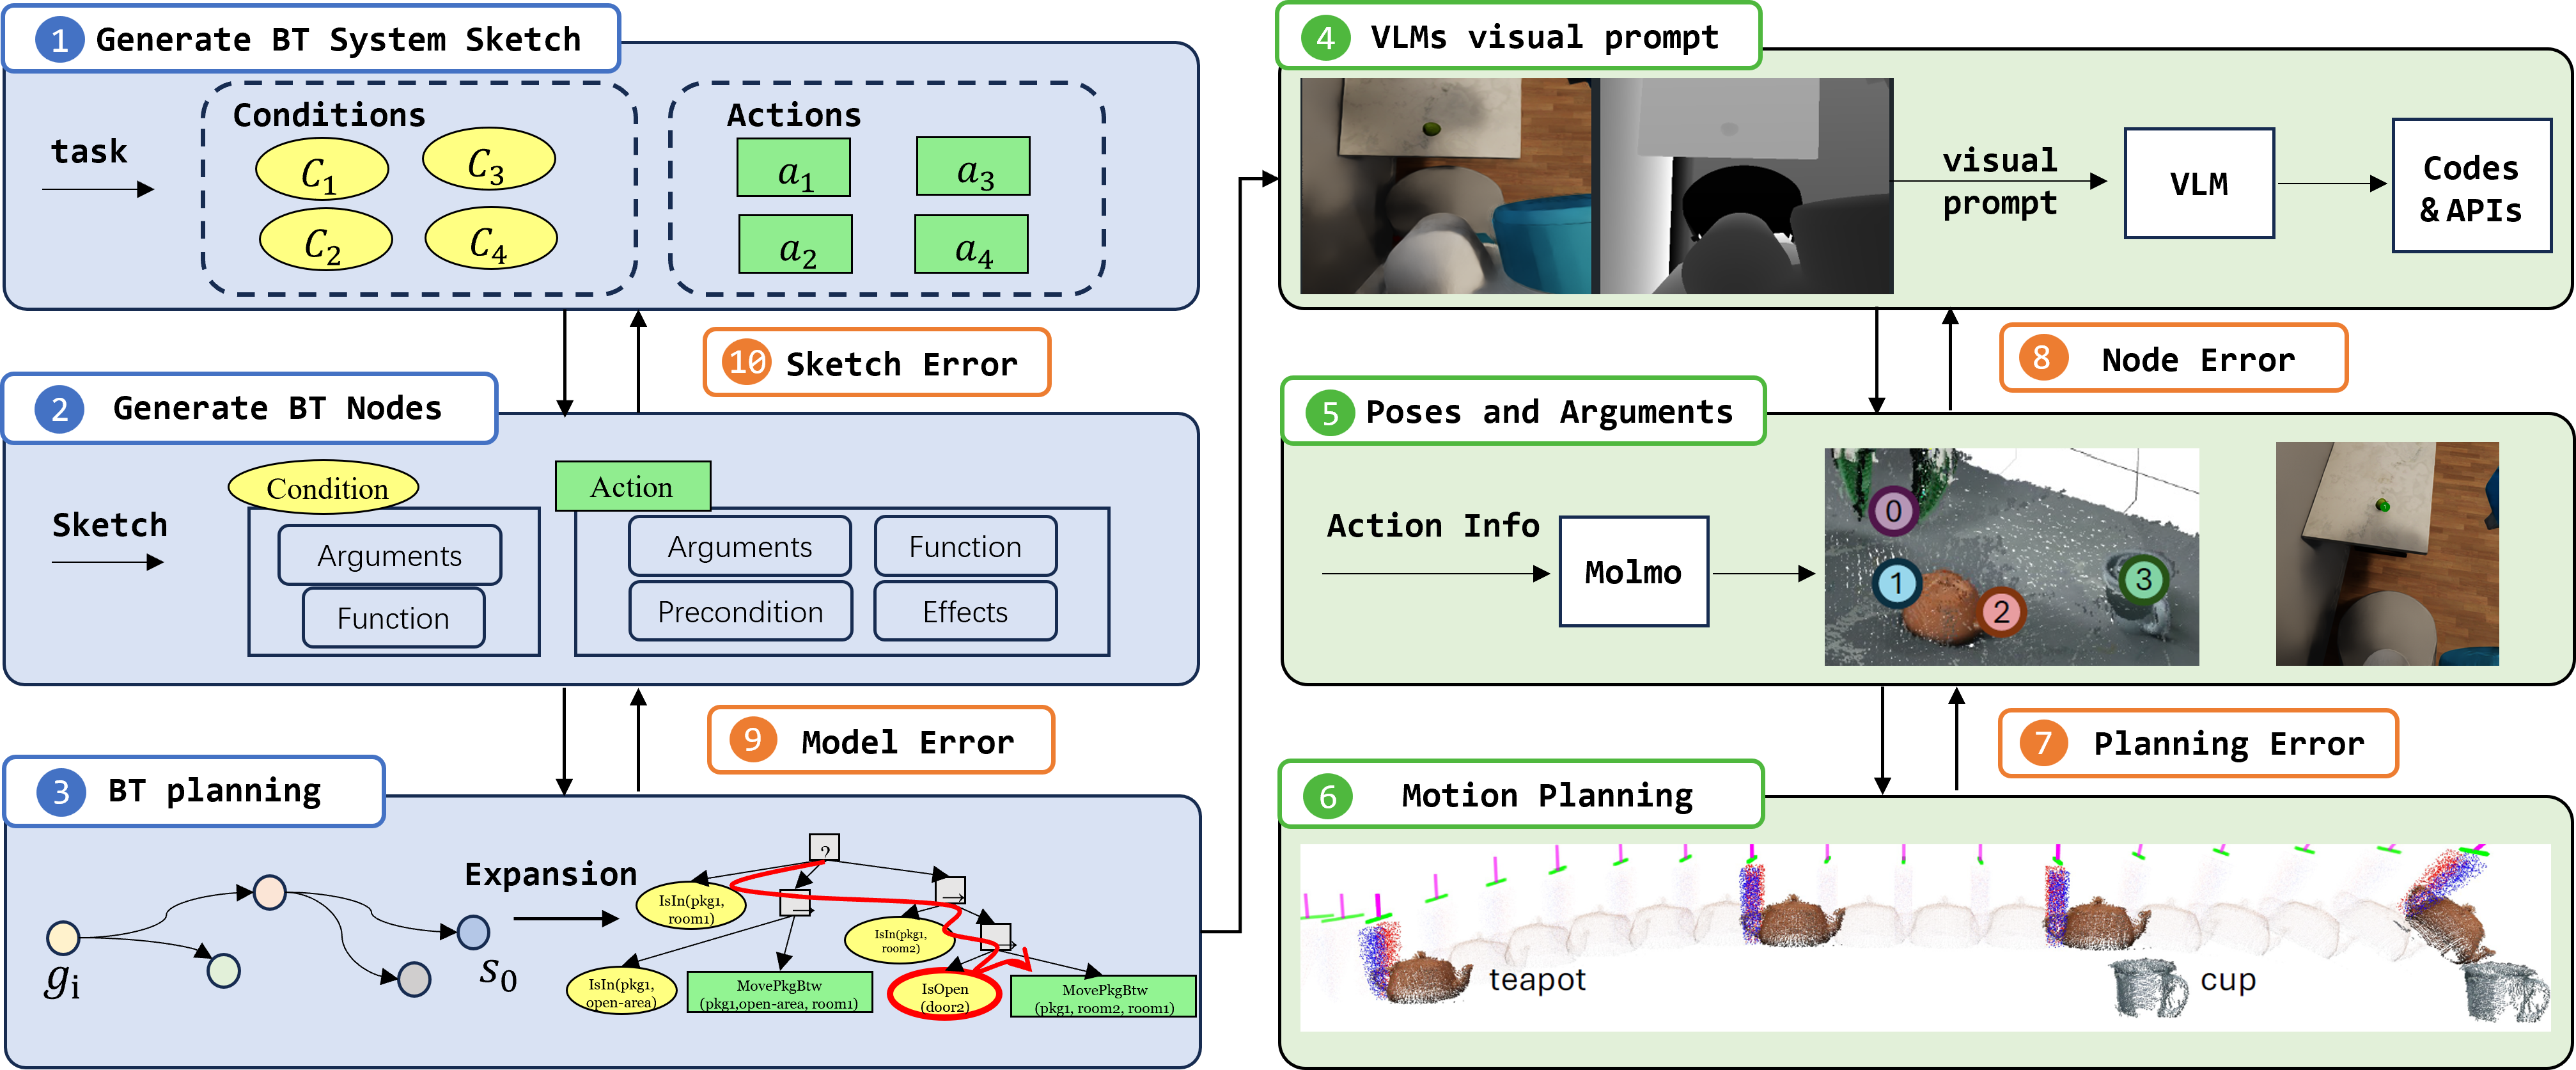
\includegraphics[width=1\textwidth]{figures/framework}
    \caption{Hierarchical robot manipulation framework with symbolic VLA.}
    \label{fig:symbolic_reasoning}
\end{figure*}




\section{Methodology}



\subsection{Overview}

Our method consists of three main components: a high-level task planner, an action chunking module, and a low-level executor. The high-level planner decomposes long-horizon tasks into subgoal sequences, the action chunking module transforms subgoals into executable action chunks, and the low-level executor carries out specific robotic actions.


\subsection{BT System Designing}

\paragraph{Generate BT system}

% 输入:task set, 采用 BDDL的格式,以及其自带的那些condition predicates,该格式来自于BEHAVIOR-1K。其中每个任务包括,objects, condition predicates, goal, s_0。然后我们只需要去生成action nodes。

% 每个action nodes包括:name, valid objects. 以及动作模型pre,add,del。还有执行的codes和APIs。prompt包括task set, condition predicates, 可行的API,few-shot templates。具体的模板见附录。LLM生成完后,我们要对输出进行解析,并为每个action生成一个class,保存至behavior libraray中。


\paragraph{Completeness validation}

% 我们使用一个sound and compelete的算法,例如BT Expasion来对我们所生成的BT system进行规划。如果所有任务均规划成功,则说明BT system是完备的。否则,说明是不完备的。

% 当不完备时,把没完成的任务挑选出来,对当前所规划出来的树结构进行摘要,然后反馈给LLM,大模型会增加新的动作节点,直到所有任务都能完成。

% lemma,第n+1次反馈后,BT 系统的完备性一定大于等于第n次。

% 证明:由于动作空间是有限的。设反馈次数为n,当n-〉inf,整个BT系统一定是->Completeness. 

% 反馈方法:对于当前所规划出的行为树,每一个叶子节点都与初始状态建立一个直接能完成的动作,比如产生10个候选。写出每个动作的pre,add,del如何定义。然后让大模型去给每个动作命名,确定参数,最后挑出前3个一致性最高的动作。

% 证明,假设为每个动作都生成一个直接完成的动作,即pre,del为空,add只有一个谓词。这样的一个BT系统一定是完备的,但不一定是一致的。

\subsection{BT Node Execution}

% 经过上面的步骤,当前行为树系统一定是完备的,但是不一定是一致的。因此我们需要在BT execution的过程中去验证完备性。

\paragraph{Keypoint Proposal}

% 现在每个任务开始执行测试。执行过程中,除了一些基于规则的API。我们最重要的一个api是Keypoint proposal。

% 这个模块采用Molmo作为VLM,其优势在于可以给图片打上基于语义的关键点。它的输入是:机器人观测到的相机图像,text包含传入的当前需要操作的物体参数,和一些物体的关键位置,以及提示词。例如对于打开抽屉,需要把点打在handle上。对于启动微波炉,要把点打在按钮上。Molmo打完点后,我们转换为世界坐标。

% 通过这个坐标,求出 eef target pose。这个pose再用motion planning的算法进行规划。如果这个pose可以达到,并且可以完成任务。


\paragraph{Consistency Validation}

% 我们根据动作的pre去生成单元测试的初始状态,并且通过add,del计算出该场景的任务目标。使用这些来采样并生成任务场景。然后将机器人置于其中进行动作的执行。我们可以得到一个N次执行的成功率。如果成功率高于一定的阈值,则认为该动作是一致的。如果成功率太低,则认为是不一致的。

% 首先pre本身有可能冲突,如果采样失败,则说明是pre本身的冲突。还有目标有可能冲突?add,del也可能有问题。其次就是pre,add,del都没有问题,但是执行的代码有问题。

% 反馈有几种情况:
% 1. molmo打点错误。用VLM改molmo的prompt。
% 2. 如果是代码错误,由于我们这篇文章不关注代码生成,我们认为API足够合理时,大模型能够正确的输出代码,如果代码不对,则简单的重新生成几遍。


\subsection{Cross-level Feedback}

% 如果底层修改多次都不对,则认为是pre,add,del错误。让大模型去增加一个新的动作pre,add,del。这个就同时涉及到 Completeness and Consistency。

% 假设pre成立,但是effect和原有的不一样。这时候不动代码,改effect。但是这时候就可能不再是完备的,所以需要重新进行Completeness validation。假设pre不成立,

% 可能会降低完备性的情况:加pre,加del,减add。
% 可能会降低一致性的情况:减pre,减del,加add。

% 不能加重复的,不能加不一致的。
% 提供一些当前场景中的信息:包括当前正在执行的动作模型,比如视觉信息,以及底层的Molmo和motion planning。 比如open(),handEmpty()。





% 假设我们可以通过一个BT system 

The inputs include: $\mathcal{T}$
We input the task information into the LLM.

A complete BT system $\Phi$ includes a condition and actions that can perform the whole tasks.

A Condition is complete if it can determine the success or failure of the task.

% 一个动作节点是良定义的,如果在任何满足precondition的s下,总是能让环境发生所定义的转移。
An Action is complete if it can perform the model.


% 一个完备的BT系统是对于所有给定的任务都可以有效完成的。每个动作都是良定义的。


% 动作的成功率。动作导致的环境转移可能是多少?在任意的情况下的总成功率?
Success Rate of Action:

% 我们就是要不断地提高动作的成功率。


\paragraph{BT Planning}

We use the sound and complete BT Expansion \cite{cai2021bt} algorithm to solve the BT. \constant{A}. 






\subsection{BT Execution}


\paragraph{VLMs visual prompt}

% 首先我们把要生成的动作信息输入给VLM,让VLM输出一段代码来控制机器人。其中我们有一些已经写好的底层API,例如移动等。
First, we input the action information we want to generate into the VLM, and let the VLM output a piece of code to control the robot. We have some pre-written low-level APIs, such as movement.

\paragraph{Poses and Constraints}

% 对于底层来说,图像处理是很重要的。我们先让molmo生成关键点,然后将关键点转换为pose。

For the lower level, image processing is very important. We first let Molmo generate keypoints, and then convert these keypoints into poses.

\paragraph{Motion Planning}

motion planning is very important. We use cuRobo to efficiently solve the problem.

\subsection{Feedback}
We use the good thing to do that.

\paragraph{Action Model Error}

% Putin失败是因为没有open.
% LLM生成placeOn的时候忘记添加IsHandEmpty。

Putin's failure is because there was no open.  
LLM forgot to add IsHandEmpty when generating placeOn.

\paragraph{Molmo Error}

% 缺少isNear,就开始Near。
% curobo失败是因为molmo打点没打对。

Missing isNear, just start Near.  
Curobo failed because Molmo's dot placement was incorrect.


% \subsection{Implementation Details}

% In our implementation, we employ the following techniques:

% \begin{itemize}
%     \item Use large language models for high-level task decomposition and action chunk selection
%     \item Train parameterized policies for action chunks using reinforcement learning
%     \item Design feedback mechanisms to handle execution failures
% \end{itemize}

% Through this hierarchical approach, our system can effectively handle complex long-horizon manipulation tasks.

\section{Experiments}

Our code is available at \href{https://anonymous.4open.science/r/CABTO}{https://anonymous.4open.science/r/CABTO}.


\subsection{Experimental Setup}

We conducted our experiments in the Omnigibson simulation environment. Omnigibson provides realistic physics simulation and rich interactive scenarios, making it ideal for evaluating long-horizon robotic manipulation tasks. We designed the following task scenarios:

\begin{itemize}
    \item Object Organization Task: Requires the robot to sort and place scattered items in designated locations
    \item Table Setting Task: Includes placing cutlery, pouring water, and other dining table preparation actions
    \item Kitchen Cooking Task: Requires following recipe steps to complete simple cooking procedures
\end{itemize}

% TODO: 设备信息


\subsection{BT System designing by LLM}

% \paragraph{Setup} 

% 我们使用了GPT-4o作为LLM。我们有5个设计好的API。例如keypoint proposal. 见附录

we first test the ability of LLM for BT system designing.




\subsection{BT Execution by VLM}

we then test the ability of VLM for BT execution.


\paragraph{Baselines}

We compared our method with the following baselines:

\begin{itemize}
    \item End-to-end reinforcement learning approach
    \item Rule-based hierarchical planning method
    \item Language model method without action chunking
\end{itemize}

\subsection{Results}

Our experimental results demonstrate significant advantages in the following aspects:

\begin{itemize}
    \item Task Completion Rate: 20\% improvement in average completion rate across all tasks
    \item Planning Efficiency: 40\% reduction in planning time compared to baseline methods
    \item Generalization: Ability to adapt to variations in object positions and shapes
\end{itemize}

Quantitative analysis shows that action chunking significantly improved system performance:

\begin{itemize}
    \item Reduced average planning steps
    \item Improved success rate of individual actions
    \item Decreased computational resource consumption
\end{itemize}

\subsection{Ablation Studies}

To validate the importance of each component, we conducted ablation studies:

\begin{itemize}
    \item Removing the action chunking module
    \item Using different language models
    \item Adjusting the number of planning hierarchies
\end{itemize}

Results confirm that action chunking is the key factor in improving system performance.


\subsection{Behavior Library Generation}


\begin{table}[h!]
\centering
\setlength{\tabcolsep}{3pt} % 调整列间距,默认为6pt
\small
\begin{tabular}{lcccccc}
\toprule
% Task & \makecell{Action Predicate \\ Count} & \makecell{Condition Predicate \\ Count} & \makecell{Expanded \\ Number} & \makecell{Success \\ Rate} \\
% \textbf{Tasks} & \textbf{\makecell{Action \\ Predicate}} & \textbf{\makecell{Condition \\ Predicate}} & \textbf{\makecell{Expanded \\ Number}} & \textbf{\makecell{Success \\ Rate}} \\

% \textbf{Tasks} & \textbf{\makecell{Acts}} & \textbf{\makecell{Conds}} & \textbf{\makecell{EN}} & \textbf{\makecell{Steps}} & \textbf{\makecell{SR \\ Open-loop}} & \textbf{\makecell{SR \\ Closed-loop}}\\

% \textbf{Tasks} & \textbf{\makecell{Acts}} & \textbf{\makecell{Conds}} & \textbf{\makecell{EN}} & \textbf{\makecell{Steps}} & \textbf{\makecell{SR-NF}} & \textbf{\makecell{SR-3F}}\\
\textbf{Tasks} & \textbf{\makecell{Acts}} & \textbf{\makecell{Conds}} & \textbf{\makecell{Expands}} & \textbf{\makecell{Steps}} & \textbf{\makecell{SR}}\\
\midrule
% 在这里添加你的数据
% 示例:
Pick \& Place & 3 & 4 & 5 & 4 &  10/10  \\
Open \& PutIn & 4 & 6 & 10 & 5 & 9/10  \\
ToggleOn \& ToggleOff  & 3 & 5 & 17 & 6 & 7/10 \\
Home Rearrangement & 6 & 7 & 122 & 10 & 6/10 \\
Meal Preparation & 6 & 7 & 411 & 11 & 5/10   \\
\midrule
\textbf{Total} & 4.4 & 5.8 & 113 & 7.2 & 74\%  \\
% 继续添加更多行
\bottomrule
\end{tabular}
\caption{Comparison of tasks based on predicate counts and accuracy.}
\label{tab:task_comparison}
\end{table}



\begin{table}[h!]
\centering
\setlength{\tabcolsep}{6pt} % 调整列间距,默认为6pt
\small
\begin{tabular}{lcccc}
\toprule
% Task & \makecell{Action Predicate \\ Count} & \makecell{Condition Predicate \\ Count} & \makecell{Expanded \\ Number} & \makecell{Success \\ Rate} \\
% Action & \makecell{SR} & \makecell{Molmo SR} & \makecell{Curobo SR} & \makecell{} \\
 % &  & \makecell{ReKep} & \makecell{CABTO} & \makecell{} \\
\textbf{Actions} & \textbf{\makecell{VoxPoser}} & \textbf{\makecell{ReKep}} & \textbf{\makecell{ReKep+Molmo}} & \makecell{} \\
\midrule
% 在这里添加你的数据
% 示例:
% Pick & 60\% (6/10) & 33.3\% (10/30) & 25\% (10/40) &  \\
% Place & 40\% (4/10) & 20\% (5/25) & 12.5\% (5/40) &  \\
% Open & 87.5\% (7/8) & 37.5\% (3/8) & 62.5\% (5/8) &  \\
% Close & 83.3\% (10/12) & 29.2\% (7/24) & 41.7\% (5/12) &  \\
% SwitchOn & 87.5\% (7/8) & 37.5\% (3/8) & 62.5\% (5/8) &  \\
% SwitchOff & 83.3\% (10/12) & 29.2\% (7/24) & 41.7\% (5/12) &  \\
Pick & 6/10 & 7/10 & 8/10 \\
Place & 5/10 & 8/10 & 8/10 \\
Open & 1/10 & 1/10 & 5/10 \\
Close & 2/10 & 3/10 & 7/10 \\
Toggle & 1/10 & 4/10 & 6/10 \\
% SwitchOn & 1/10 & 4/10 & 6/10 \\
% SwitchOff & 8/10 & 3/10 & 4/10 \\
\midrule
\textbf{Total} & 30\% & 46\% & 68\% &   \\
% 继续添加更多行
\bottomrule
\end{tabular}
\caption{Comparison of tasks based on predicate counts and accuracy.}
\label{tab:task_comparison}
\end{table}



% \begin{table}[h!]
% \centering
% \setlength{\tabcolsep}{3pt} % 调整列间距,默认为6pt
% \small
% \begin{tabular}{lccccc}
% \toprule
% % Task & \makecell{Action Predicate \\ Count} & \makecell{Condition Predicate \\ Count} & \makecell{Expanded \\ Number} & \makecell{Success \\ Rate} \\
%  &  & \multicolumn{3}{c}{\textbf{CABTO(Ours)}}\\
% \cline{3-5}
% \rule{0pt}{2.5ex}
% \makecell{\textbf{Tasks}} & \makecell{\textbf{ReKep}} & \makecell{SR-NF} & \makecell{SR-F} & \makecell{Feedback Times}\\
% \midrule
% % 在这里添加你的数据
% % 示例:
% {Place Apple} & 6/10 & 6/10 & 4 (2+2)  \\
% {Put Pen in Drawer} & - & 5/10 & 5 (2+3) \\
% {Activate Two Lights} & - & 4/10 & 5 (3+2)  \\
% {Home Rearrangement} & - &  3/10 & 5 (3+2)  \\
% {Meal Preparation} & - & 2/10 & 5 (3+2)  \\
% \midrule
% \textbf{Total} & ???\% & ???\% & ???\%    \\
% \bottomrule
% \end{tabular}
% \caption{Comparison of tasks based on predicate counts and accuracy.}
% \label{tab:task_comparison}
% \end{table}

\begin{table}[h!]
\centering
\setlength{\tabcolsep}{6pt} % 调整列间距,默认为6pt
\small
\begin{tabular}{lcccc}
\toprule
\makecell{\textbf{Tasks}} & \makecell{SR-NF} & \makecell{SR-F} & \makecell{Feedbacks}\\
\midrule
% 在这里添加你的数据
% 示例:
% {Case1} & 5/10 & ?/10 & 4 (2+2)  \\
{Case1: } & {} & ?/10 & 5 (2+3) \\
{Case2: } & {} & ?/10 & 5 (2+3) \\
{Case3: } & {} & ?/10 & 5 (2+3) \\
% {Activate Two Lights} &  2/10 & ?/10 & 5 (3+2)  \\
% {Home Rearrangement} &  2/10 & ?/10 & 5 (3+2)  \\
% {Meal Preparation} &  1/10 & ?/10 & 5 (3+2)  \\
\midrule
\textbf{Total} & ???\% & ???\% & ???\%    \\
\bottomrule
\end{tabular}
\caption{Comparison of tasks based on predicate counts and accuracy.}
\label{tab:task_comparison}
\end{table}


\begin{table}[h!]
\centering
\setlength{\tabcolsep}{3pt} % 调整列间距,默认为6pt
\small
\begin{tabular}{lcccccc}
\toprule
\textbf{Tasks} & \textbf{\makecell{High-level}} & \textbf{\makecell{Molmo-level}} & \textbf{\makecell{Cross-level}}\\
\midrule
Pick \& Place & 1 & 5 & 0  \\
Open \& PutIn & 2 & 7 & 3  \\
ToggleOn \& ToggleOff  & 4 & 5 & 0 \\
Home Rearrangement & ? & ? & ?\\
Meal Preparation & ? & ? & ?  \\
\textbf{Total} &  &  &    \\
% 继续添加更多行
\bottomrule
\end{tabular}
\caption{Comparison of tasks based on predicate counts and accuracy.}
\label{tab:task_comparison}
\end{table}


\subsection{Behavior Library Excution}


apple



\section{Related Work}


\subsection{Behavior Tree Generation}
Current BT generation methods are usually focused on generating the BT's structure with well designed BT systems. Various methods have been explored for this purpose. Heuristic search methods, such as grammatical evolution \cite{neupane2019learning}, genetic programming \cite{colledanchise2019learning,lim2010evolving}, and Monte Carlo DAG Search \cite{scheide2021behavior}, have been widely investigated. 
In addition to heuristic approaches, machine learning techniques have been applied to generate BTs. In particular, methods such as reinforcement learning \cite{banerjee2018autonomous,pereira2015framework} and imitation learning \cite{french2019learning} have gained attention. 
There are also research efforts that employ formal synthesis methods to generate BTs, such as Linear Temporal Logic (LTL) \cite{li2021reactive} and its variant approaches \cite{tadewos2022specificationguided,neupane2023designing}.


\subsection{VLA}

VLA is proven to be effective and efficient for robotic manipulation tasks \cite{li2024generalist}.  

There are many papers use end-to-end VLA architecture for robotic manipulation \cite{kim2024openvla,wen2024tinyvla,zhen20243dvla}. Meanwhile, there are some papers use hierarchical VLA architecture for robotic navigation \cite{chiang2024mobility} and manipulation \cite{huang2024rekep}.

code generation for robot manipulation is a good way to achieve long-horizon manipulation tasks.\cite{mu2024robocodex}

Skill-based reinforcement learning is a good way to achieve long-horizon manipulation tasks.\cite{haresh2024clevrskills}



\subsection{Symbolic Grounding for Robot Manipulation}

current atom action has several ways to be grounded.

\begin{itemize}
    \item Rule-based grounding. \cite{yang2024guiding,yang2025octopus} use optimization-based trajectory planning. First only use the subgoal-related object to generate the trajectory, if the trajectory is not feasible, then add the other objects to the trajectory. While $N_{TAMP}$ failures, the trajectory is not feasible.
    \item VLM-based constraint generation. These methods often use the VLM to output the spatial-temporal constraints and combines the low-level motion planner to achieve long-horizon visual planning \cite{huang2024rekep}. \cite{kumar2024openworld} use VLM to output the discrete and continuous constraints. \cite{liu2024moka} uses VLM to generate affordance based on keypoints
\end{itemize}



There are some papers use VLM to output spatial-temporal constraints and combines the low-level motion planner to achieve long-horizon visual planning \cite{huang2024rekep,zhou2024codeasmonitor}.


\subsection{Code for Robot Manipulation}

some papers generate code for robot manipulation \cite{mu2024robocodex}. But these papers are not suitable for long-horizon manipulation tasks.

However, the current architecture of code generation for robot manipulation is not suitable for long-horizon manipulation tasks.

There are some paper use policy to directly control the robot, such as grasp \cite{wang2023dexgraspnet}. However, they face the problem of sim2real gap.


some paper uses VLM to output spatial-temporal constraints and combines the low-level motion planner to achieve long-horizon visual planning.
\cite{huang2024rekep,zhou2024codeasmonitor} however, these papers limited to the acurracy of keypoint labeling, which is not easy to achieve in real-world tasks.


guided the low-level motion planner with fine-grained eef-pose is a good way to achieve long-horizon manipulation tasks.

\subsection{Action Chunking}

Action chunking is a concept in cognitive science and robotics that refers to the process of grouping primitive actions into larger, meaningful units.

This concept is inspired by how humans learn and execute complex motor skills.

We don't think about individual muscle movements, but rather in terms of higher-level action sequences.

In the context of robotic manipulation, action chunking helps to:

\begin{itemize}
    \item Reduce the complexity of long-horizon tasks by breaking them down into manageable sub-sequences
    \item Enable more efficient learning by allowing the robot to reuse common action patterns
    \item Bridge the gap between high-level task planning and low-level motion control
\end{itemize}

For example, instead of planning each individual joint movement for picking up an object, a chunked action might combine reaching, grasping, and lifting into a single "pick" action chunk. This hierarchical representation makes planning more tractable and allows for better generalization across similar tasks.



\section{Conclusion}

This paper presents Context-Aware Behavior Tree grOunding (CABTO), a novel framework that automates the design and grounding of BT systems based on task and execution contexts. CABTO integrates LLMs, formal algorithms, and VLMs to achieve generalization and reliability in BT planning and execution. Experiments on four household scenarios and ten manipulation tasks with the Fetch robot demonstrate its effectiveness. CABTO reduces the reliance on expert knowledge, enhances adaptability, and provides a robust solution for automated BT system grounding and task execution. Future work will focus on extending CABTO to more complex environments and improving its efficiency and scalability.







\newpage


%% The file named.bst is a bibliography style file for BibTeX 0.99c
\bibliographystyle{named}
\bibliography{strings,my_references}

\end{document}

